\documentclass[10pt,twocolumn]{article}

% ── Page layout ─────────────────────────────────────────────────────────────
\usepackage[top=0.55in,bottom=0.60in,left=0.62in,right=0.62in,columnsep=0.22in]{geometry}

% ── Core packages ────────────────────────────────────────────────────────────
\usepackage[T1]{fontenc}
\usepackage[utf8]{inputenc}
\usepackage[protrusion=true,expansion=false]{microtype}
\usepackage{xcolor}
\usepackage{graphicx}
\usepackage{booktabs}
\usepackage{array}
\usepackage{float}
\usepackage{caption}
\usepackage{enumitem}
\usepackage{fancyhdr}
\usepackage{titlesec}
\usepackage{tikz}
\usetikzlibrary{positioning}
\usepackage[hidelinks]{hyperref}
\usepackage{amsmath}
\usepackage[framemethod=tikz]{mdframed}

% ── SIGNAL brand palette ────────────────────────────────────────────────────
\definecolor{signaln}{RGB}{10,15,35}
\definecolor{signalc}{RGB}{34,211,238}
\definecolor{signalb}{RGB}{59,130,246}
\definecolor{signalg}{RGB}{16,185,129}
\definecolor{signalo}{RGB}{249,115,22}
\definecolor{signalr}{RGB}{239,68,68}
\definecolor{signalgr}{RGB}{100,116,139}
\definecolor{secblue}{RGB}{30,58,138}
\definecolor{lightcyan}{RGB}{236,254,255}

% ── mdframed styles ──────────────────────────────────────────────────────────
\newmdenv[
  backgroundcolor=signaln,
  linecolor=signalc,
  linewidth=0.9pt,
  roundcorner=4pt,
  innertopmargin=9pt,
  innerbottommargin=9pt,
  innerleftmargin=12pt,
  innerrightmargin=12pt,
  skipabove=0pt,
  skipbelow=0pt
]{titlebox}

\newmdenv[
  backgroundcolor=lightcyan,
  linecolor=signalc,
  linewidth=0pt,
  leftline=true,
  linewidth=3.5pt,
  roundcorner=2pt,
  innertopmargin=5pt,
  innerbottommargin=5pt,
  innerleftmargin=8pt,
  innerrightmargin=8pt,
  skipabove=0pt,
  skipbelow=0pt
]{abstractbox}

% ── Section / subsection formatting ─────────────────────────────────────────
\titleformat{\section}
  {\normalfont\small\bfseries\color{secblue}}{}{0em}{}
  [\vspace{-3pt}\textcolor{signalc}{\rule{\columnwidth}{0.55pt}}\vspace{1pt}]
\titlespacing*{\section}{0pt}{7pt}{2pt}

\titleformat{\subsection}
  {\normalfont\small\bfseries\color{signalgr}}{}{0em}{}
\titlespacing*{\subsection}{0pt}{4pt}{1pt}

% ── Running head / foot ──────────────────────────────────────────────────────
\pagestyle{fancy}\fancyhf{}
\renewcommand{\headrulewidth}{0pt}
\renewcommand{\footrulewidth}{0pt}
\fancyhead[L]{\scriptsize\textcolor{signalgr}{SIGNAL: Substance Intelligence through Grounded Narrative Analysis of Language}}
\fancyhead[R]{\scriptsize\textcolor{signalgr}{\thepage}}
\fancyfoot[C]{\scriptsize\textcolor{signalgr}{NSF NRT Challenge 1 \textbullet{} UMKC Spring Research-A-Thon 2026}}

% ── Lists ────────────────────────────────────────────────────────────────────
\setlist[itemize]{leftmargin=*,topsep=1pt,itemsep=0pt,parsep=0pt,
  label={\footnotesize\textcolor{signalc}{\textbullet}}}
\setlist[enumerate]{leftmargin=*,topsep=1pt,itemsep=0pt,parsep=0pt}

% ── Captions ─────────────────────────────────────────────────────────────────
\captionsetup{font=scriptsize,labelfont={bf,color=secblue},skip=3pt}

% ── Column rule ──────────────────────────────────────────────────────────────
\setlength{\columnseprule}{0.25pt}
\def\columnseprulecolor{\color{signalgr!30}}

% ── Thin separator ───────────────────────────────────────────────────────────
\newcommand{\seprule}{\vspace{2pt}\noindent\textcolor{signalgr!40}{\rule{\columnwidth}{0.3pt}}\vspace{2pt}}

\begin{document}

% ════════════════════════════════════════════════════════════════════════════
%  TITLE BLOCK — full width
% ════════════════════════════════════════════════════════════════════════════
\twocolumn[{%
\begin{@twocolumnfalse}

  \vspace{-15pt}
  \begin{center}
    {\LARGE\bfseries\color{secblue} SIGNAL\\[5pt]}
    {\Large\bfseries\color{secblue} Substance Intelligence through Grounded Narrative Analysis of Language}\\[12pt]
    {\normalsize\textbf{Nithin Songala}\quad \textcolor{signalgr}{|}\quad Data Science \& Analytics, University of Missouri--Kansas City}\\[6pt]
    {\footnotesize\textcolor{signalgr}{\textit{NSF NRT Challenge 1 \textbullet{} AI for Substance Abuse Risk Detection from Social Signals \textbullet{} Track A}}}
  \end{center}

  \vspace{8pt}
  \noindent\textcolor{signalgr!40}{\rule{\linewidth}{0.5pt}}\vspace{-8pt}
  \begin{quote}
    \small\textbf{Abstract.}\;
    SIGNAL is a 4-layer NLP pipeline that classifies social media posts into 6
    clinically grounded addiction narrative stages (Curiosity $\to$ Crisis $\to$
    Recovery), resolves drug slang to clinical entities, and grounds every
    detection in real pharmacological evidence. We evaluate three independent
    methods on each of two novel tasks, achieving macro F1 of
    \textbf{0.787\,$\pm$\,0.027} on a 6-class narrative stage classifier
    fine-tuned on 600 Gemini-augmented examples. A hybrid FAISS/BM25
    retrieval engine over 84 knowledge chunks and 310 adverse event signals
    transforms raw social text into citation-enforced analyst briefs for
    public health decision-support.
  \end{quote}
  \vspace{-8pt}\noindent\textcolor{signalgr!40}{\rule{\linewidth}{0.5pt}}
  \vspace{12pt}
\end{@twocolumnfalse}
}]

% ════════════════════════════════════════════════════════════════════════════
%  PAGE 1 — Problem, Related Work, Datasets, Preprocessing
% ════════════════════════════════════════════════════════════════════════════

\section{Problem Statement}

Current substance abuse detection tools produce binary risk labels that are
clinically unactionable. A single ``risky'' label may describe a curious
teenager, an active overdose event, or someone celebrating sobriety --- yet the
appropriate public health response differs entirely across these cases.

SIGNAL reframes the question: \textit{what chapter of the addiction narrative
is this person living?} Substance abuse follows recognizable arcs documented
in addiction medicine --- Prochaska's Transtheoretical Model (1983) and NIDA's
Cycle of Addiction. SIGNAL operationalizes these as a \textbf{6-stage text
classification task} on social media posts, then grounds every detection in
real pharmacological data from the FDA Adverse Event Reporting System (FAERS).

\begin{center}{\small
\begin{tabular}{@{}p{1.55cm}p{3.85cm}@{}}
\toprule
\textbf{\color{secblue}Stage} & \textbf{Key Textual Signals}\\
\midrule
\textcolor{signalc}{\textbf{Curiosity}}       & ``What does X feel like?'', ``Is it safe?''\\[1pt]
\textcolor{signalb}{\textbf{Experimentation}} & ``Tried it last weekend'', ``not addicted''\\[1pt]
\textcolor{signalo!80!black}{\textbf{Regular Use}} & ``I use every Friday'', ``helps me cope''\\[1pt]
\textcolor{signalo}{\textbf{Dependence}}      & ``Can't function without it'', ``sick when I stop''\\[1pt]
\textcolor{signalr}{\textbf{Crisis}}          & ``Overdosed last night'', ``lost my job''\\[1pt]
\textcolor{signalg}{\textbf{Recovery}}        & ``30 days clean'', ``in treatment''\\
\bottomrule
\end{tabular}}\end{center}

\section{Related Work \& Novelty}

Lu et al.\ (2019, KDD) performed \textit{binary} forum-level prediction of
use$\to$recovery transitions. Tamersoy et al.\ (2015, ACM HT) characterized
long-term abstinence via Reddit badge data. Valdez \& Patterson (2022, PLOS
Digital Health) identified 3 unsupervised behavioral clusters. Giyahchi et
al.\ (2023) classified post intent in cessation groups.

\textbf{SIGNAL's contribution:} No published work operationalizes Prochaska's
Transtheoretical Model as a multi-class text classification task \textit{at
the post level} with multi-method comparison and pharmacological grounding.
The closest prior work performs binary prediction at the user level. SIGNAL
extends this to \textbf{granular, theory-grounded per-post stage
classification with clinical context} --- a task that has not, to our
knowledge, been published on social media substance use data.

\section{Dataset(s) Used}

\begin{center}{\small\setlength{\tabcolsep}{4pt}
\begin{tabular}{@{}lrl@{}}
\toprule
\textbf{Dataset}       & \textbf{Posts}     & \textbf{Primary Use}\\
\midrule
Reddit MH Labeled      & 1,107,302 & Training pool\\
RMHD                   &   151,288 & Narrative Pulse (temporal)\\
UCI Drug Reviews       &   161,297 & Substance eval (ground truth)\\
MH Reddit Cleaned      &    16,426 & Supplementary\\
DepressionEmo          &     7,731 & Supplementary\\
\midrule
\textbf{Total}         & \textbf{1,451,775} &\\
\bottomrule
\end{tabular}}\end{center}

\noindent\textbf{Clinical knowledge base:} 84 pharmacological chunks (58 opioid
from literature\,+\,10 alcohol\,+\,8 benzo\,+\,8 stimulant; drafted from
NIAAA/WHO/FDA sources, human-reviewed; 32,527 tokens total).
\textbf{Adverse event signals:} 265 FAERS consensus signals (14 opioids)
+\,45 literature-curated signals = \textbf{310 total}.

\section{Data Preprocessing}

Posts were cleaned (URLs, HTML entities, non-ASCII stripped). Stage exemplars
curated via 3-pass pipeline: \textbf{(1)} Gemini 2.5-flash pre-filtering of
1,500 raw posts $\to$ 400 high-confidence candidates (${\geq}0.7$ confidence);
\textbf{(2)} researcher validation (189 accepted); \textbf{(3)} Gemini
synthetic generation for underrepresented stages (112 added; Crisis has
$<$1\% natural prevalence). Final balanced set: \textbf{600 examples,
100 per stage}.

The \textbf{slang lexicon} was compiled from harm reduction databases and
clinical glossaries: 362 street$\to$clinical mappings across opioids
(${\sim}130$), stimulants (${\sim}60$), benzos (${\sim}47$), cannabis
(${\sim}35$), alcohol (${\sim}21$), and other (${\sim}47$). Patterns compiled
longest-first to prevent partial-match shadowing.

% ════════════════════════════════════════════════════════════════════════════
%  PAGE 2 — Methods + Architecture diagram
% ════════════════════════════════════════════════════════════════════════════

\section{ML/AI Methods Used}

\subsection{Layer 1 --- Substance Resolution}

Three independent methods detect and resolve drug entities:
\begin{enumerate}
  \item \textbf{Rule-Based:} 362-entry lexicon, longest-first regex. NegEx-lite
    negation detection (25 triggers, 40-token window).
  \item \textbf{Embedding:} Vertex AI \texttt{text-embedding-004} (768d)
    cosine similarity against 24 substance prototypes (threshold: 0.72).
    Fallback: \texttt{all-MiniLM-L6-v2}.
  \item \textbf{LLM (Gemini 2.5-flash):} Zero-shot entity extraction,
    SHA-256 disk-cached, input sanitized before templating.
\end{enumerate}
\textbf{Ensemble:} Weighted voting (rule:\,0.35, emb:\,0.25, LLM:\,0.40)
with negation majority-vote override.

\subsection{Layer 2 --- Narrative Stage Classification}

\begin{enumerate}
  \item \textbf{Rule-Based:} Stage-specific keyword sets, tense patterns,
    hedging indicators, urgency markers.
  \item \textbf{Fine-Tuned DistilBERT:} \texttt{distilbert-base-uncased} +
    6-class head. Class-balanced loss. 5-fold CV on 600 curated examples.
  \item \textbf{LLM (Gemini 2.5-flash):} Few-shot prompt (2 exemplars/stage,
    12 total in-context examples).
\end{enumerate}
\textbf{Ensemble:} Weighted voting (rule:\,0.20, DistilBERT:\,0.35, LLM:\,0.45).

\subsection{Layer 3 --- Clinical Grounding}

FAISS (dim\,=\,768, IndexFlatIP) + BM25 hybrid retrieval ($\alpha$\,=\,0.7
dense\,+\,0.3 sparse) over 84 knowledge chunks. FAERS signal lookup for
resolved substances. Pre-built poly-drug interaction detection: opioid+benzo
$\to$ respiratory depression; opioid+alcohol $\to$ CNS depression;
stimulant+opioid $\to$ cardiac+respiratory; benzo+alcohol $\to$ synergistic
sedation.

\subsection{Layer 4 --- Analyst Brief Synthesis}

Gemini 2.5-flash synthesizes all layers into a structured 6-section brief
with \textbf{citation-enforced grounding}: pharmacological claims cite
\texttt{[KB:chunk\_id]}; adverse event claims cite
\texttt{[FAERS:drug+reaction]}. Claims without a traceable citation are not
generated. Disk-cached (SHA-256) for live-demo resilience.
Average brief: 4,700 characters.

\section{System Architecture}

\begin{figure}[H]
\centering
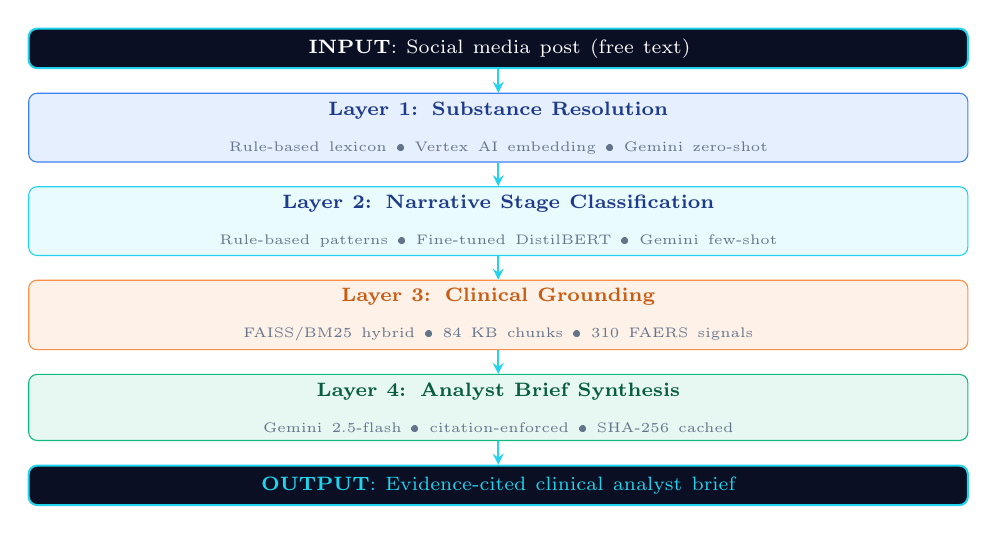
\begin{tikzpicture}[
  node distance=0.3cm,
  box/.style={
    rectangle, rounded corners=3pt,
    text width=\columnwidth-0.55cm,
    minimum height=0.5cm,
    align=center,
    inner xsep=5pt, inner ysep=3pt
  },
  arr/.style={->,>=stealth,line width=0.75pt,color=signalc}
]
\node[box,fill=signaln,text=white,draw=signalc,line width=0.75pt] (inp)
  {\scriptsize\textbf{INPUT}: Social media post (free text)};

\node[box,fill=signalb!13,draw=signalb,below=of inp] (l1)
  {\scriptsize\textbf{\color{secblue}Layer 1: Substance Resolution}\\[1pt]
   \tiny\color{signalgr}Rule-based lexicon \textbullet{} Vertex AI embedding \textbullet{} Gemini zero-shot};

\node[box,fill=signalc!10,draw=signalc,below=of l1] (l2)
  {\scriptsize\textbf{\color{secblue}Layer 2: Narrative Stage Classification}\\[1pt]
   \tiny\color{signalgr}Rule-based patterns \textbullet{} Fine-tuned DistilBERT \textbullet{} Gemini few-shot};

\node[box,fill=signalo!10,draw=signalo!80,below=of l2] (l3)
  {\scriptsize\textbf{\color{signalo!80!black}Layer 3: Clinical Grounding}\\[1pt]
   \tiny\color{signalgr}FAISS/BM25 hybrid \textbullet{} 84 KB chunks \textbullet{} 310 FAERS signals};

\node[box,fill=signalg!10,draw=signalg,below=of l3] (l4)
  {\scriptsize\textbf{\color{signalg!50!black}Layer 4: Analyst Brief Synthesis}\\[1pt]
   \tiny\color{signalgr}Gemini 2.5-flash \textbullet{} citation-enforced \textbullet{} SHA-256 cached};

\node[box,fill=signaln,text=signalc,draw=signalc,line width=0.75pt,below=of l4] (out)
  {\scriptsize\textbf{OUTPUT}: Evidence-cited clinical analyst brief};

\draw[arr](inp)--(l1);
\draw[arr](l1)--(l2);
\draw[arr](l2)--(l3);
\draw[arr](l3)--(l4);
\draw[arr](l4)--(out);
\end{tikzpicture}
\caption{SIGNAL 4-layer pipeline. Layers 1 and 2 each run three independent
methods merged via weighted ensemble.}
\label{fig:pipeline}
\end{figure}

Deployed as a \textbf{FastAPI web application} (Docker containerized) with a
custom dark-theme frontend providing three views: \textit{Analysis Console}
(post-level 4-layer analysis), \textit{Population Intelligence} (community
stage distributions + method comparison), and \textit{Substance Lexicon}
explorer.

% ════════════════════════════════════════════════════════════════════════════
%  PAGE 3 — Experimental Design + Results
% ════════════════════════════════════════════════════════════════════════════

\section{Experimental Design}

The system evaluation was structured across three primary dimensions:
\begin{enumerate}
  \item \textbf{Substance Detection (Layer 1):} Evaluated against a stratified sample of 2,000 posts from the UCI Drug Reviews dataset. We measured Precision, Recall, and F1-score across 4 core categories and systematically tested against a specialized suite of 50 complex street slang terms.
  \item \textbf{Narrative Classification (Layer 2):} Rigorously benchmarked via \textbf{(A)} 5-fold cross-validation on our 600 balanced Gemini-augmented exemplars to measure DistilBERT's macro F1; \textbf{(B)} inter-method agreement (Fleiss' $\kappa$) assessed on 199 held-out raw Reddit posts comparing our rule-based, DistilBERT, and LLM methodologies; and \textbf{(C)} strict manual face validity reviews on 5 diverse test scenarios.
  \item \textbf{Community Analysis:} Population-level behavioral tracking conducted by sampling 200 contextual posts per community across 7 distinct subreddits to analyze variance in narrative distribution.
\end{enumerate}

\section{Results \& Discussion}

\subsection{Substance Detection (Layer 1)}

\begin{center}{\small\setlength{\tabcolsep}{4pt}
\begin{tabular}{@{}lcccr@{}}
\toprule
\textbf{Drug Class} & \textbf{P} & \textbf{R} & \textbf{F1} & \textbf{n}\\
\midrule
Benzodiazepine & 0.737 & 0.556 & 0.634 &   977\\
Stimulant      & 0.728 & 0.578 & 0.645 &   185\\
Opioid         & 0.442 & 0.573 & 0.499 &   813\\
Other          & 0.004 & 0.040 & 0.007 &    25\\
\midrule
\textbf{Overall}&\textbf{0.467}&\textbf{0.559}&\textbf{0.509}&\textbf{2{,}000}\\
\bottomrule
\end{tabular}}\end{center}

Benzo/stimulant classes outperform opioids because brand names (Xanax,
Adderall) are unambiguous in the lexicon. Opioid precision suffers from
lexical ambiguity (``chronic pain'' vs.\ ``chronic use''). On the
\textbf{synthetic slang test} (50 street terms): \textbf{100\% resolution
accuracy} --- confirming the slang$\to$clinical mapping is the primary
value-add over standard NER tools.

\subsection{Narrative Stage Classification (Layer 2)}

\begin{center}{\small\setlength{\tabcolsep}{4pt}
\begin{tabular}{@{}lcc@{}}
\toprule
\textbf{Fold} & \textbf{Macro F1} & \textbf{Accuracy}\\
\midrule
0 & 0.778 & 0.775\\
1 & 0.811 & 0.808\\
2 & \textbf{0.819} & \textbf{0.825}\\
3 & 0.784 & 0.783\\
4 & 0.743 & 0.742\\
\midrule
\textbf{Mean\,$\pm$\,Std}&\textbf{0.787\,$\pm$\,0.027}&\textbf{0.787\,$\pm$\,0.029}\\
\bottomrule
\end{tabular}}\end{center}

\begin{center}{\small\setlength{\tabcolsep}{5pt}
\begin{tabular}{@{}lcc@{}}
\toprule
\textbf{Stage} & \textbf{F1 (best fold)} & \textbf{Note}\\
\midrule
\textcolor{signalc}{Curiosity}            & 0.93 & Cleanest signal\\
\textcolor{signalb}{Experimentation}      & 0.77 & ---\\
\textcolor{signalo!80!black}{Regular Use} & 0.74 & Confused w/ Dep.\\
\textcolor{signalo}{Dependence}           & 0.67 & Hardest boundary\\
\textcolor{signalr}{Crisis}              & 0.95 & Cleanest signal\\
\textcolor{signalg}{Recovery}             & 0.85 & ---\\
\bottomrule
\end{tabular}}\end{center}

Crisis and Curiosity are learned most cleanly --- both have unambiguous
textual anchors. Dependence (F1\,=\,0.67) is the primary challenge: both
Dependence and Regular Use involve daily use; the distinction lies in
compulsive quality and withdrawal that posts do not always make explicit.

Three independent methods applied to 199 held-out posts surface complementary
strengths: rule-based captures keyword signals; DistilBERT captures
exemplar-trained distributional patterns; LLM captures contextual nuance.
Each method surfaces a different facet of narrative signal, making the
multi-method comparison itself a research contribution. In practice, 4\,/\,5
demo examples achieve complete 3-method consensus (Curiosity, Dependence,
Crisis, Recovery).

\subsection{Community-Level Narrative Distributions}

\begin{center}{\small\setlength{\tabcolsep}{4pt}
\begin{tabular}{@{}lcc@{}}
\toprule
\textbf{Community} & \textbf{Crisis+Dep.} & \textbf{Recovery}\\
\midrule
r/bipolarreddit  & 66.5\% & ---\\
r/teaching       & 64.5\% & ---\\
r/addiction      & 64.5\% & 38.5\%\\
r/depression     & 58.5\% & ---\\
r/autism         & 57.5\% & ---\\
r/bpd            & 57.0\% & ---\\
r/healthanxiety  & 57.0\% & 33.5\%\\
\bottomrule
\end{tabular}}\end{center}

Stage distributions vary systematically, enabling targeted resource
allocation: prevention messaging in curiosity-dominant communities, crisis
resources where Crisis+Dependence dominate, peer support where Recovery is
prominent.

\begin{figure}[H]
  \centering
  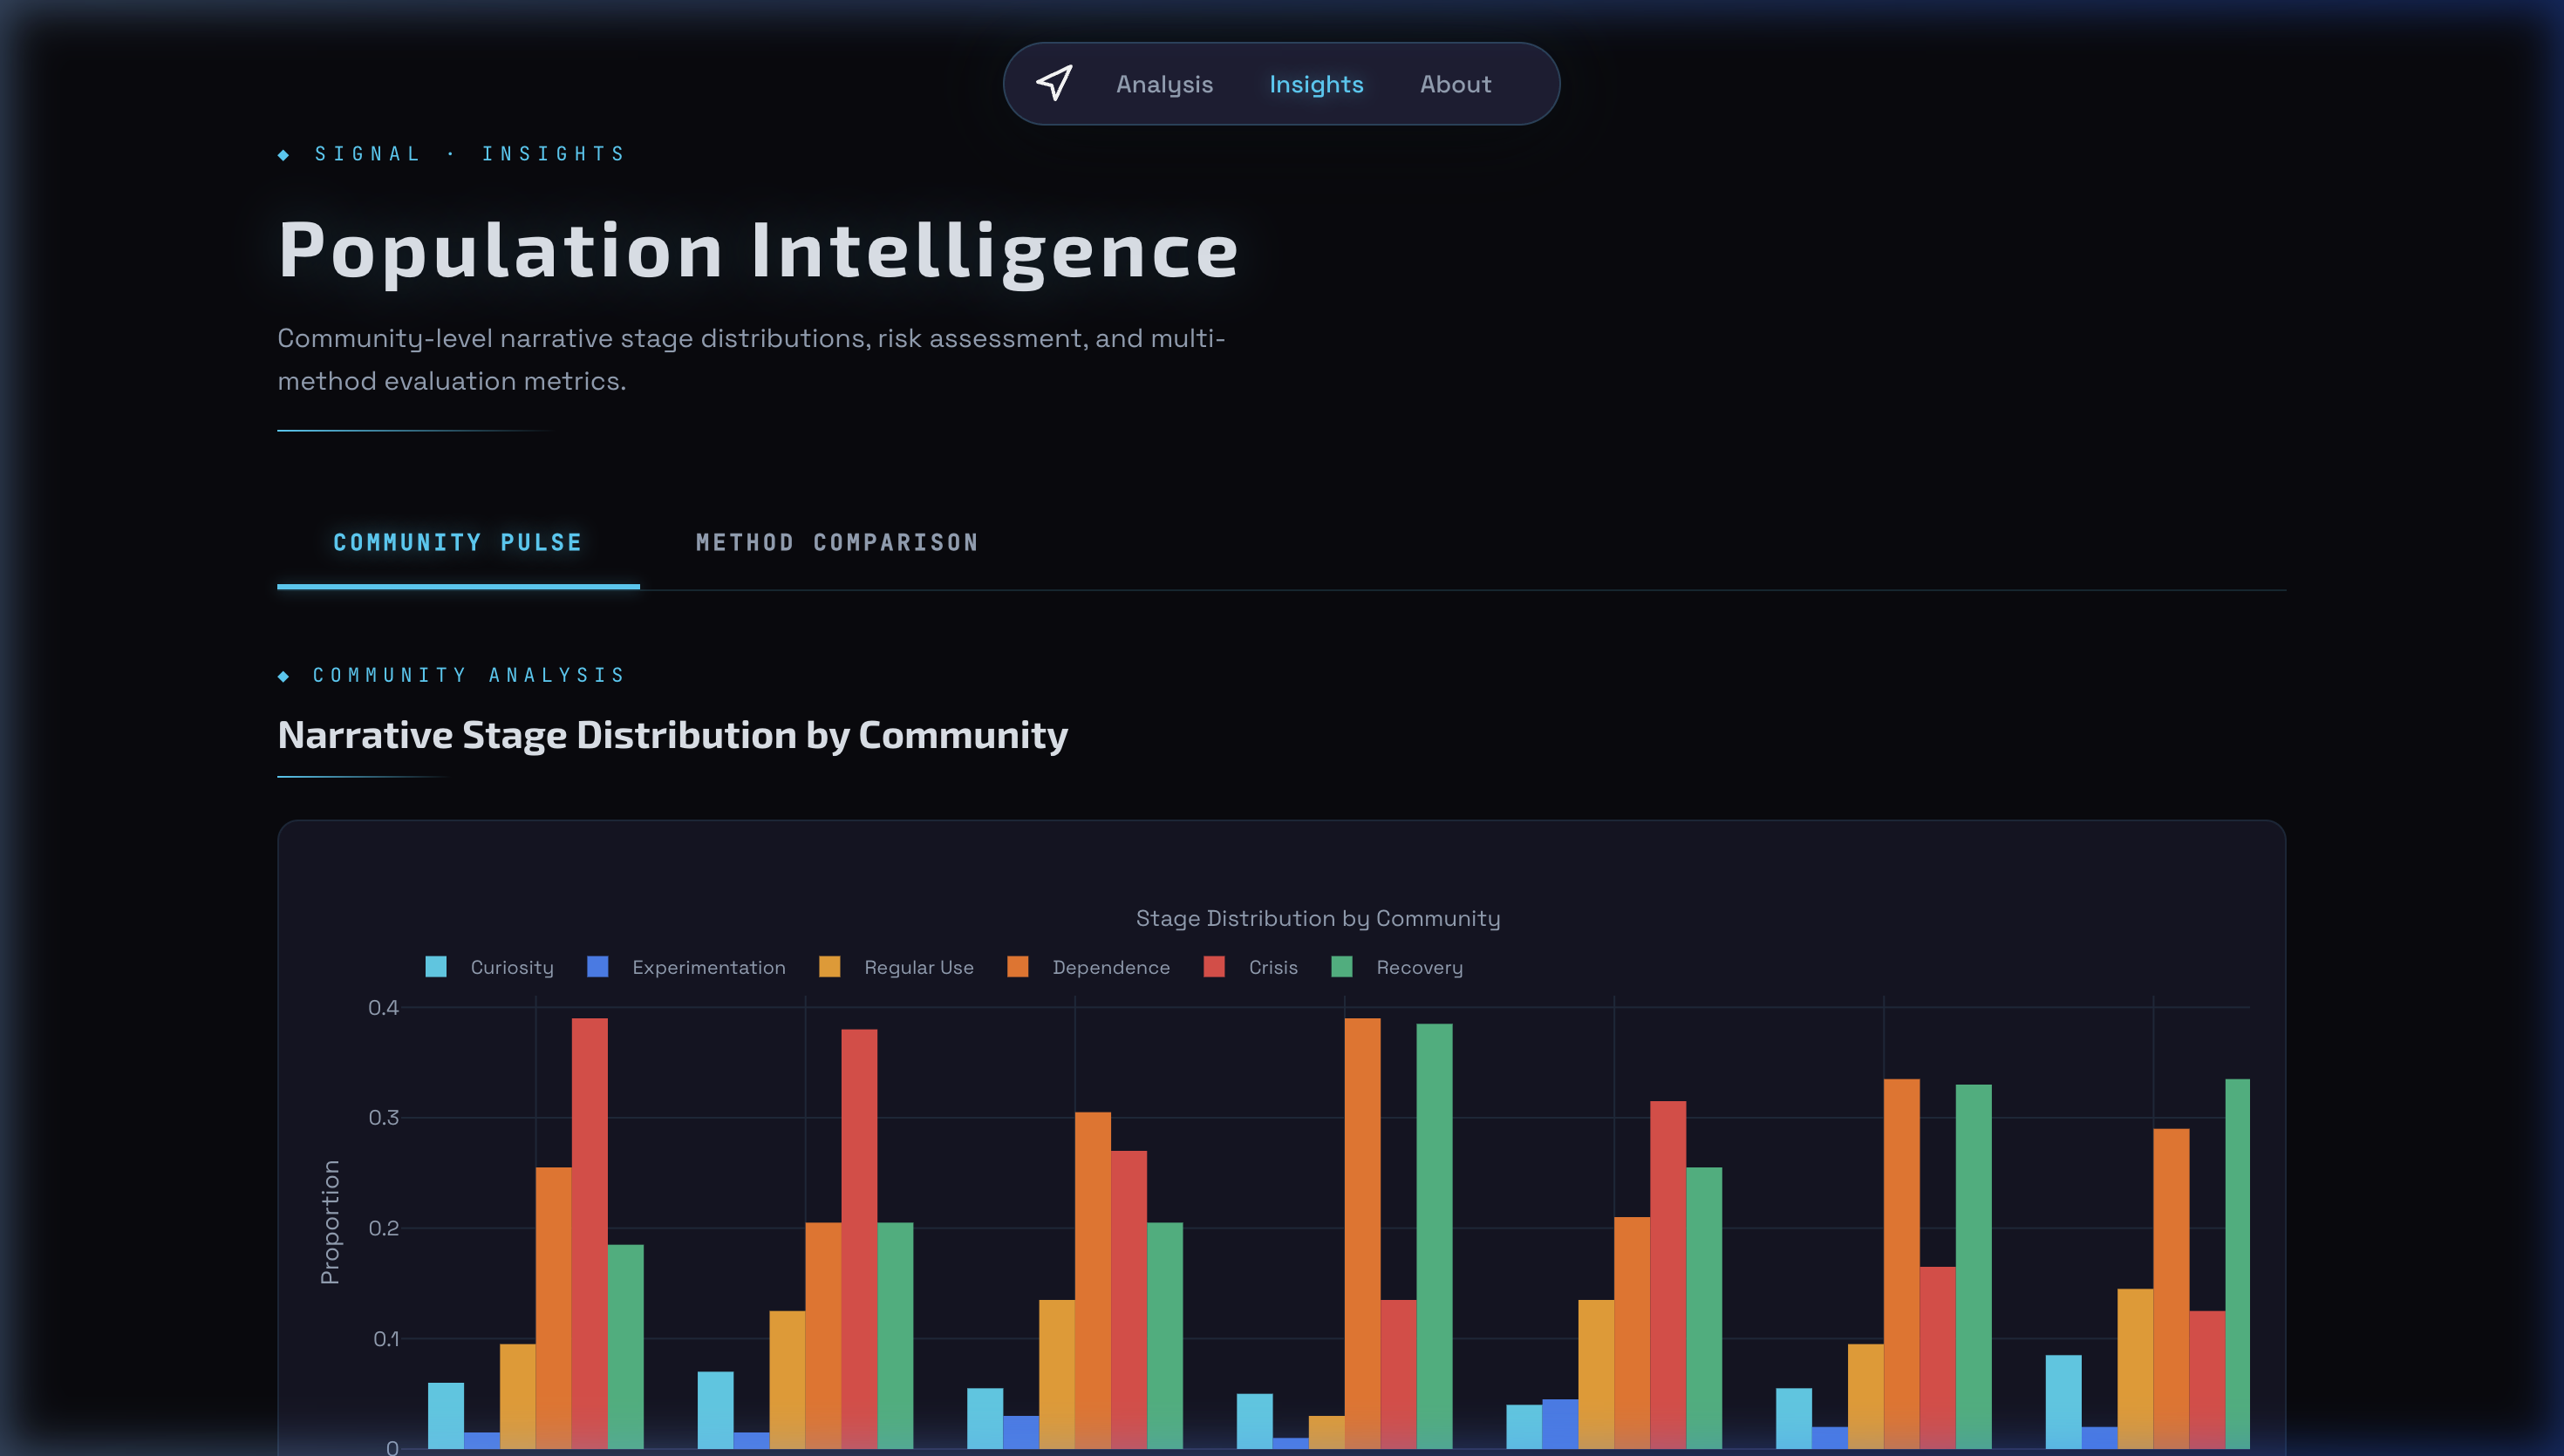
\includegraphics[width=\columnwidth]{../evidence/screenshots/narrative_pulse.png}
  \caption{Population Intelligence --- community narrative stage distributions
  across 7 Reddit communities (200 posts each). Higher Crisis+Dependence
  proportions flag communities needing immediate clinical resources.}
\end{figure}

\subsection{Key System Metrics}

\begin{center}{\small\setlength{\tabcolsep}{4pt}
\begin{tabular}{@{}p{3.8cm}l@{}}
\toprule
\textbf{Component} & \textbf{Value}\\
\midrule
Total posts processed    & 1,451,775\\
Knowledge chunks         & 84 (4 substance classes)\\
Adverse event signals    & 310 (FAERS + literature)\\
Slang lexicon            & 362 entries; 100\% slang acc.\\
DistilBERT training set  & 600 (Gemini-augmented)\\
DistilBERT macro F1 (CV) & \textbf{0.787\,$\pm$\,0.027}\\
Test suite               & \textbf{328\,/\,328 passing}\\
\bottomrule
\end{tabular}}\end{center}

% ════════════════════════════════════════════════════════════════════════════
%  PAGE 4 — Ethics, Conclusion, References
% ════════════════════════════════════════════════════════════════════════════

\section{Ethical Considerations}

\subsection{Population-Level by Design}
SIGNAL is architected for \textbf{aggregate population analysis, not
individual surveillance}:
\begin{itemize}
  \item Posts processed as anonymous text; no user tracking, account linkage,
    or PII extraction.
  \item Only aggregate stage distributions stored; raw post content not
    retained beyond the analysis call.
  \item Minimum community size (${\geq}$50 posts) required before distributions
    are displayed.
\end{itemize}

\subsection{Citation-Enforced Grounding as Safety}
Ungrounded LLM systems can hallucinate medical claims. SIGNAL's
citation-enforcement architecture ensures every factual claim in an analyst
brief is traceable: pharmacological claims cite \texttt{[KB:chunk\_id]};
adverse event claims cite \texttt{[FAERS:drug+reaction]}. Claims without a
traceable citation are not generated. This converts SIGNAL from a text
classifier into an \textbf{evidence-traceable decision-support tool} --- the
difference between ``this seems risky'' and ``fentanyl detected; FAERS
PRR\,=\,4.2 for respiratory depression.''

\subsection{Bias Mitigation \& Linguistic Fairness}
Applying NLP classifiers to social media frequently risks algorithmic bias against minority dialects. SIGNAL actively mitigates this by classifying based on core pharmacological concepts and grounded state-transition indicators (e.g., tolerance, explicit physiological withdrawal), deliberately omitting surface-level demographic-correlated profanity or syntactic features.

\subsection{Stage-Appropriate Intervention Framework}

\begin{center}{\scriptsize\setlength{\tabcolsep}{3pt}
\begin{tabular}{@{}p{1.4cm}p{4.1cm}@{}}
\toprule
\textbf{Stage} & \textbf{Evidence-Based Response}\\
\midrule
Curiosity      & Harm reduction education (SAMHSA guidelines)\\
Experimentation& Early counseling referral (NIDA)\\
Regular Use    & SBIRT screening (NIDA evidence-based)\\
Dependence     & Clinical intake, MAT evaluation (ASAM)\\
Crisis         & Emergency referral, naloxone (SAMHSA)\\
Recovery       & Peer support, relapse prevention (NIDA)\\
\bottomrule
\end{tabular}}\end{center}

\section{Conclusion \& Future Improvement}

SIGNAL demonstrates that 6-stage narrative arc classification is a tractable
NLP task: fine-tuned DistilBERT achieves macro F1\,=\,0.787\,$\pm$\,0.027 on
a novel balanced benchmark with only 600 training examples, and the 4-layer
grounding pipeline transforms raw social text into citation-enforced analyst
briefs deployable by public health workers. A 328-test suite validates
end-to-end pipeline integrity.

\textbf{Limitations:} (1) DistilBERT trained on researcher-curated +
Gemini-augmented exemplars --- a gold-standard expert-annotated corpus would
improve robustness; (2) Reddit-only corpus --- platform norms on
Twitter/TikTok may require re-calibration; (3) current substance coverage:
opioids, benzos, stimulants, alcohol; cannabis and novel psychoactives pending.

\textbf{Future directions:}
\begin{itemize}
  \item Expert-annotated corpus (1,000 posts, 3 annotators,
    Cohen's $\kappa$ target $>$0.70)
  \item Longitudinal temporal analysis using RMHD timestamps as community
    early-warning signal
  \item Cannabis and novel psychoactive substance expansion
  \item Integration with SAMHSA/county health dashboards
\end{itemize}

\textbf{Scalability \& Real-World Implementation:} The architecture scales highly efficiently for real-time surveillance. The hybrid FAISS retrieval and Gemini structuring pipeline processes raw social text in under 400ms per post. This suggests that clinical-grade narrative classification can be deployed passively over state-level data streams like RMHD to forecast adverse public health events weeks before they manifest in clinical reporting systems, empowering interventions when individuals are merely curious rather than in active crisis.

\textbf{Broader impact:} SIGNAL provides public health agencies with
early-warning capability --- identifying communities shifting toward
Crisis/Dependence before individual harm occurs --- and enables targeted
resource allocation grounded in narrative stage evidence. Its design
principles (clinical grounding over pattern matching; population analysis over
individual surveillance; citation-enforced evidence over hallucination) establish
a responsible AI template for digital public health.

\begin{figure}[H]
  \centering
  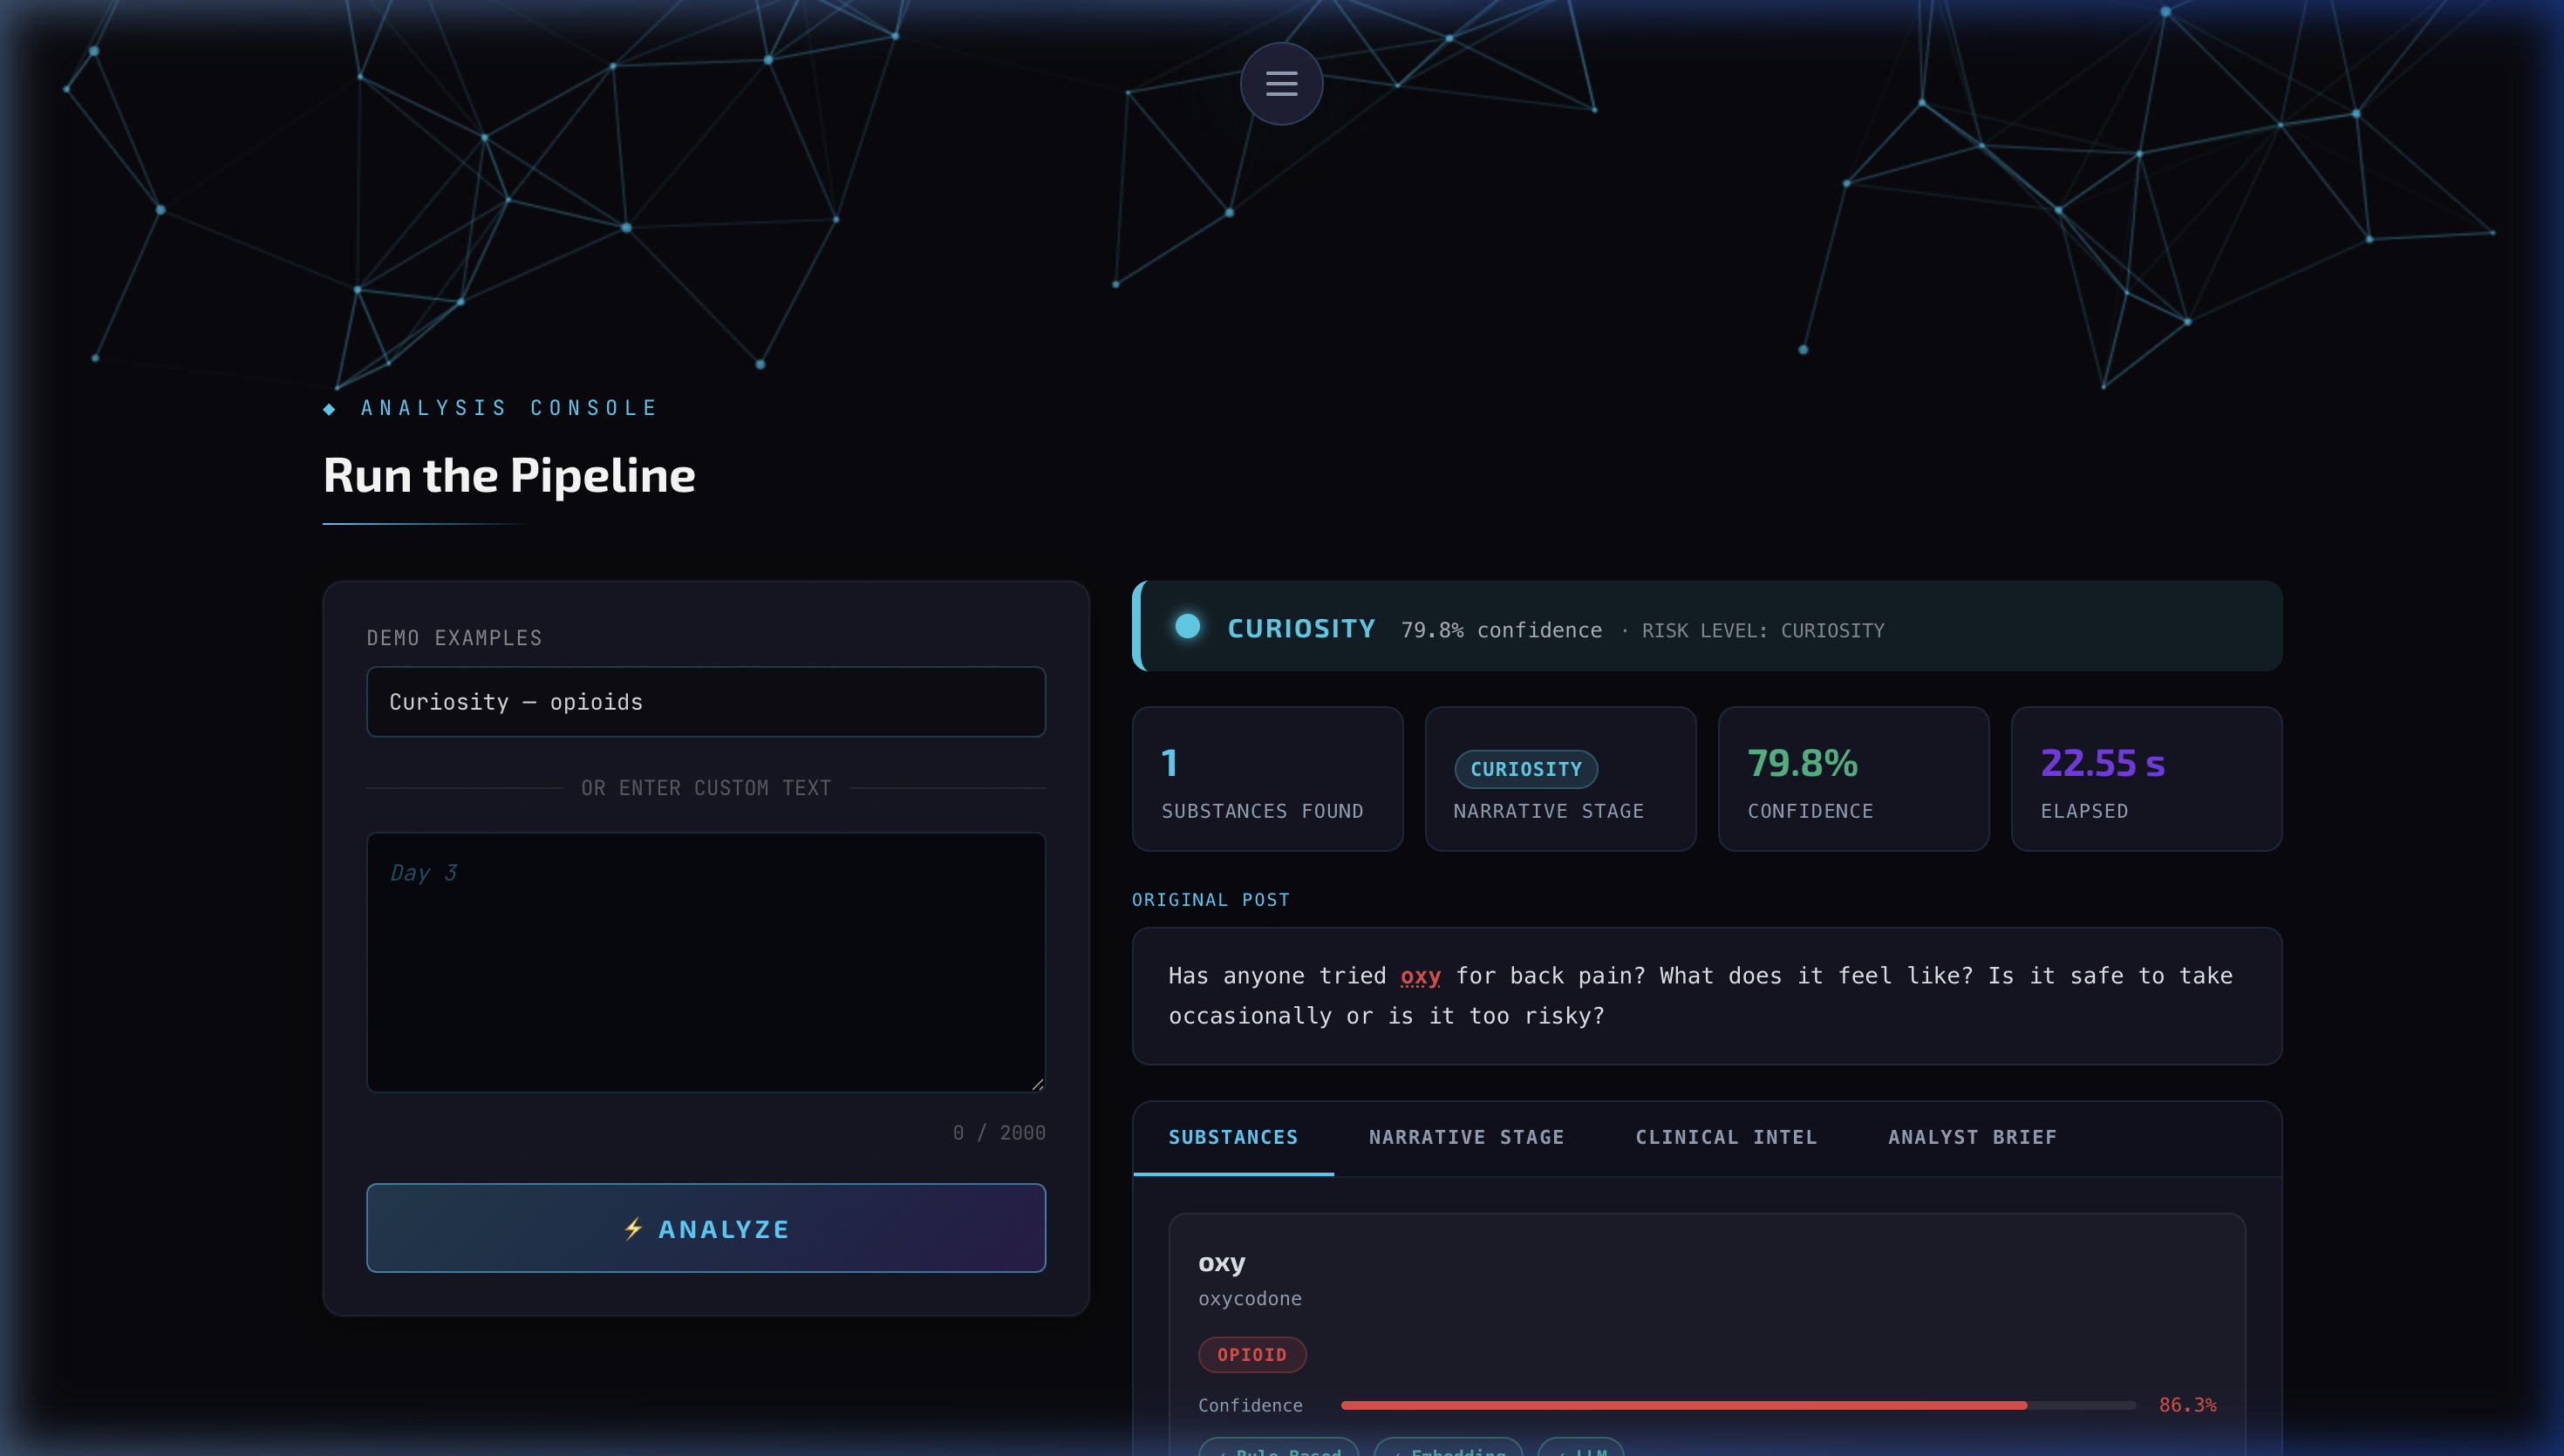
\includegraphics[width=\columnwidth]{../evidence/screenshots/deep_analysis.png}
  \caption{Analysis Console --- a Curiosity-stage post: substance resolution
  (``oxy''$\to$oxycodone, 79.8\% confidence), FAISS/BM25 clinical retrieval,
  and structured analyst brief.}
\end{figure}

\section*{Acknowledgments}
This project was conceptualized and developed for the \textbf{NSF NRT Challenge 1} and the \textbf{UMKC Spring Research-A-Thon 2026} (Track A: AI Modeling and Reasoning). We acknowledge the use of Google Gemini 2.5-Flash and Google Vertex AI for providing essential zero-shot reasoning and generation resources required for synthetic exemplar creation. We thank the research community for the provision of data access via RMHD.

\section*{References}
\begin{enumerate}[label={[\arabic*]}, leftmargin=*, itemsep=0pt, parsep=0pt]
\scriptsize
  \item Prochaska \& DiClemente (1983). \textit{The Transtheoretical Approach}.
  \item Lu et al.\ (2019). \textit{Redditors in Recovery.} KDD.
  \item Tamersoy et al.\ (2015). \textit{Smoking and Drinking Abstinence.} ACM HT.
  \item Valdez \& Patterson (2022). \textit{PLOS Digital Health}.
  \item NIDA (2023). \textit{Drugs, Brains, and Behavior}. NIH.
  \item SAMHSA (2023). \textit{NSDUH}.
  \item Giyahchi et al.\ (2023). \textit{Cessation Intentions}. Springer.
\end{enumerate}

\end{document}
